\documentclass[conference]{IEEEtran}
\usepackage[utf8]{inputenc}
\usepackage{amsmath,amssymb,graphicx,booktabs}

\usepackage[hidelinks,unicode,pdftitle={Validation-Selected Linear Interpolation Between Qwen2.5-0.5B Base and Instruct: Does It Beat Both Parents on ARC, HellaSwag and WinoGrande?},pdfauthor={Dheiver Francisco Santos},pdfkeywords={model merging, weight interpolation, Qwen2.5, instruction tuning, paired bootstrap, negative result},pdfsubject={Preprint, Figshare, doi:10.6084/m9.figshare.35013979}]{hyperref}
\begin{document}

\title{Validation-Selected Linear Interpolation Between Qwen2.5-0.5B Base and Instruct: Does It Beat Both Parents on ARC, HellaSwag and WinoGrande?}

\author{\IEEEauthorblockN{Dheiver Francisco Santos, PhD}
\IEEEauthorblockA{Independent Researcher\\
Maceió, Alagoas, Brazil\\
ORCID: https://orcid.org/0000-0002-8599-9436\\
Preprint, Figshare, 2026, \href{https://doi.org/10.6084/m9.figshare.35013979}{doi:10.6084/m9.figshare.35013979}, CC BY 4.0}}

\maketitle

\begin{abstract}
Interpolating the weights of a pretrained model and its fine-tuned sibling has beaten both endpoints in some vision settings. We ask whether the same holds for a small language model. We interpolate linearly between Qwen2.5-0.5B and Qwen2.5-0.5B-Instruct on eleven coefficients, choose $t^\ast$ on 300 validation items per task, and report it on 3{,}967 disjoint test items from ARC-Easy, ARC-Challenge, HellaSwag and WinoGrande. The pre-registered criterion was a paired 95\% bootstrap interval for the gain over the better original model lying entirely above zero. It was not met. The selected $t^\ast=0.7$ reaches 50.90\% test accuracy against 50.25\% for the base model, a difference of $+0.65$ pp (95\% CI $[-0.23,+1.52]$, $p=0.149$): a tie. The Spearman rank correlation between validation and test accuracy over the eleven coefficients is $\rho=-0.03$ ($p=0.93$), so the validation split carried no detectable information about the test ranking. By this selection procedure and this test set, gains above about 1.5 pp are excluded; smaller gains are neither confirmed nor excluded. One model pair and four benchmarks limit generality.
\end{abstract}

\begin{IEEEkeywords}
model merging, weight interpolation, Qwen2.5, instruction tuning, paired bootstrap, negative result
\end{IEEEkeywords}

\section{Introduction}
Open small language models are usually released as a pair: a base checkpoint and an instruction-tuned checkpoint that start from the same weights. Because the two share an initialization, their parameters can be combined in weight space without any training. The simplest combination is linear interpolation (LERP) with one scalar $t$, which costs one weighted sum and one evaluation per candidate $t$. Prior work on robust fine-tuning of vision models reports that intermediate coefficients can exceed both endpoints \cite{wortsman2022wise}. It is less clear whether this transfers to a sub-billion-parameter language model. It is also unclear whether the gain survives a clean separation between the data used to choose $t$ and the data used to report it.

This paper tests one pre-registered hypothesis. For Qwen2.5-0.5B base and Instruct, an interior coefficient $t^\ast$ chosen on validation items only should give a higher test macro accuracy on ARC-Easy, ARC-Challenge, HellaSwag and WinoGrande than the better original model. The lower limit of the paired 95\% confidence interval must lie above zero. ``Beating both parents'' therefore means beating the better original model as chosen on validation, which implies beating both on validation; on test it counts only if the paired interval lies above zero. Our contributions are modest. We give (i) a complete eleven-point interpolation curve on validation and test with item-level bootstrap intervals; (ii) a paired comparison against the original model chosen on validation, not on test; and (iii) the null result, including how little the validation split discriminates between coefficients.

\section{Related Work}
\textbf{Interpolation and connectivity.} Frankle et al.\ showed that networks that are stable to SGD noise are linearly connected in loss after early training \cite{frankle2020lmc}, on vision models (MNIST, ResNet, Inception); we read this as motivation for evaluating a straight line between two checkpoints. Averaging along a single training trajectory widens optima and improves generalization \cite{izmailov2018swa}. Model soups average models fine-tuned from the same initialization with different hyperparameters \cite{wortsman2022soups}. The closest antecedent is WiSE-FT, which interpolates the weights of the zero-shot and fine-tuned models and reports large robustness gains under distribution shift while preserving target accuracy \cite{wortsman2022wise}. Rewarded soups interpolate weights fine-tuned on different rewards to trace a Pareto front \cite{rame2023rewarded}. Spherical interpolation, introduced for quaternion rotations, follows an arc rather than the chord and is a common alternative for weights \cite{shoemake1985slerp}.

\textbf{Heavier merging machinery.} When models do not share an initialization, models that do not share an initialization can be merged after permutation alignment \cite{ainsworth2023rebasin}. Fisher-weighted averaging weights each parameter by its estimated importance \cite{matena2022fisher}, and dataless knowledge fusion merges language models in weight space \cite{jin2023dataless}. Task arithmetic, TIES and DARE operate on differences from the base and are introduced in \cite{ilharco2023taskarith,yadav2023ties,yu2024dare} and covered in a survey \cite{yang2024survey}; a second survey covers weight-averaging and mode-connectivity-based fusion \cite{li2023fusion}; a study of merging at larger scale reports how base-model strength changes merge quality \cite{yadav2024scale}. Chat Vector adds the difference between a chat model and its base to another model \cite{huang2023chatvector}. Toolkits such as MergeKit make these recipes routine \cite{goddard2024mergekit}.

\textbf{Evaluation under selection.} Choosing a coefficient on one split and reporting on another is a form of adaptive analysis, and adaptive reuse of a holdout can bias estimates \cite{dwork2015adaptive}. Miller argues that evals should report standard errors \cite{miller2024errorbars}.

\textbf{Gap.} We are not aware of a paired, split-separated measurement of this question for small language models. This paper fills that gap for one concrete and widely used pair, and reports the answer even though it is null.

\textbf{Author's related work.} The author's technical notes cover neighboring topics in language-model training: model merging for capability composition \cite{santos2026modelmergingfo}, knowledge distillation and self-distillation \cite{santos2026knowledgedisti}, parameter-efficient fine-tuning (LoRA, QLoRA, DoRA) \cite{santos2026parametereffic}, mixture-of-experts training and sparse upcycling \cite{santos2026mixtureofexper}, curriculum learning and data-efficient pretraining \cite{santos2026curriculumlear}, synthetic data generation and self-improvement \cite{santos2026syntheticdatag}, direct preference optimization \cite{santos2026directpreferen}, RLAIF and Constitutional AI \cite{santos2026rlaifandconsti}, and RLVR and GRPO for reasoning \cite{santos2026reinforcementl}. This paper instead reports a controlled held-out measurement. In a different domain, the author's JEPA preprint \cite{santos2026collapseresist} uses a similar controlled-comparison style (identical budgets, several seeds, confidence intervals).

\section{Method}
Let $\theta_b$ and $\theta_i$ be the parameter vectors of the base and instruct models, which have identical architecture and tokenizer. The interpolated model is
\begin{equation}
\theta(t)=(1-t)\,\theta_b+t\,\theta_i,\qquad t\in[0,1].
\end{equation}
Every tensor (embeddings, attention, MLP, norms) is interpolated with the same $t$. The merge is computed in fp32 on CPU and copied into the bf16 model used for scoring.

\subsection*{Equations and their meaning}
\textbf{Eq.~(1)} is a straight line in weight space: $t=0$ returns the base model, $t=1$ the instruct model, and $t=0.5$ their midpoint.

Let $A_s(t)$ be the accuracy of $\theta(t)$ on task $s$ and $\mathrm{M}(t)=\frac14\sum_{s}A_s(t)$ the macro average over the four tasks, so each task counts equally regardless of its size:
\begin{equation}
t^\ast=\arg\max_{t\in\mathcal{G}}\ \mathrm{M}^{\mathrm{val}}(t),\qquad \mathcal{G}=\{0,0.1,\dots,1\}.
\end{equation}
The coefficient is picked by the highest validation macro accuracy; test items are never consulted for this choice. The original model to beat is
\begin{equation}
t_o=\arg\max_{t\in\{0,1\}}\ \mathrm{M}^{\mathrm{val}}(t),
\end{equation}
that is, the better of base and instruct as judged on validation, not on test. The quantity of interest is
\begin{equation}
\Delta=\mathrm{M}^{\mathrm{test}}(t^\ast)-\mathrm{M}^{\mathrm{test}}(t_o),
\end{equation}
the paired test-set gain of the selected merge over the better parent. The maximum is taken over the whole grid, endpoints included; the hypothesis concerns an interior coefficient, and here $t^\ast=0.7$ is interior. Success means the 95\% bootstrap interval of $\Delta$ is entirely above zero; if it contains zero the outcome is a tie. The interval comes from resampling items with replacement within each task, keeping the same items for both models (paired), recomputing the macro difference, and taking the 2.5th and 97.5th percentiles.

\section{Experimental Protocol}
\textbf{Models.} Qwen2.5-0.5B (base, Hub revision \texttt{060db6499f32}) and Qwen2.5-0.5B-Instruct (\texttt{7ae557604adf}) \cite{qwen2024qwen25}, both Apache-2.0. Full 40-character hashes are in \texttt{MANIFEST.json}. The instruct model is scored with the same raw prompts as the base model, without a chat template.

\textbf{Data and splits.} ARC-Easy, ARC-Challenge \cite{clark2018arc}, HellaSwag \cite{zellers2019hellaswag} and WinoGrande \cite{sakaguchi2020winogrande}. ARC-Challenge validation is the full official validation split (299 items); its test split is subsampled from 1{,}172 to 1{,}000 items. ARC-Easy is subsampled from 570 to 300 validation items and from 2{,}376 to 1{,}000 test items. The subsamples are drawn by permutation with seed 0 (\texttt{common/evalkit.py}). HellaSwag and WinoGrande use their validation sets, partitioned into disjoint validation and test parts with seed 0. Validation has 300 items per task (299 for ARC-Challenge, which has only 299 validation items); test has 1{,}000 items per task (967 for WinoGrande), 3{,}967 in total. Scoring is by log-likelihood of each answer choice in the style of the LM Evaluation Harness \cite{gao2023harness}: length-normalized by characters for ARC-Easy, ARC-Challenge and HellaSwag, and partial scoring without normalization for WinoGrande.

\textbf{Selection.} All eleven grid points are scored on validation and $t^\ast$ is fixed by Eq.~(2) before looking at test. For the plotted curve we also scored every grid point on test; no choice depends on those numbers. Evaluation is deterministic (no training, no sampling), so there are no random seeds; the only randomness is the bootstrap (seed 0) and the seed-0 data split. Hardware is Apple Silicon (MPS), bf16; PyTorch 2.8.0, transformers 4.57.6.

\textbf{Baselines.} The primary baseline is the better original model by validation, which is the base model ($t_o=0$; validation 49.53\% against 48.53\% for instruct). We also report $t^\ast$ against $t=1$. As the ablation that isolates the interpolation, the full grid shows every other coefficient with the same budget of eleven validation evaluations.

\textbf{Statistics.} Accuracy intervals: 95\% percentile bootstrap \cite{efron1979bootstrap} over items (2{,}000 resamples, tasks resampled separately and averaged). Paired differences: 3{,}000 resamples with the same items for both models, two-sided $p$ from the bootstrap distribution (B=3,000: the smallest nonzero two-sided $p$ is 2/3,000). Six primary comparisons were declared across Articles 1--6 of this series; this paper contributes one of them. The pre-registration (\texttt{experiments/PREREG.md}) fixed 5,000 bootstrap resamples; the analysis used 2,000 for a single accuracy and 3,000 for paired differences. The Bonferroni threshold $0.05/6=0.0083$ over the six primary comparisons of this series' Articles 1--6 was added after the pre-registration, whose success rule was a paired 95\% CI above zero.

\section{Results}
Table~\ref{tab:lerp} gives the whole curve and Fig.~\ref{fig:lerp} plots it. The base model scores 50.25\% on test; the instruct model 50.64\%. The validation-selected $t^\ast=0.7$ scores 50.90\%.

\begin{table*}[!t]
\caption{Qwen2.5-0.5B base ($t=0$) to instruct ($t=1$) interpolation. Macro accuracy (\%) with 95\% bootstrap CI on validation ($n\approx300$ per task) and test ($n\approx1000$ per task); paired difference on test against the base model, which is the better original on validation, with 95\% CI and nominal two-sided $p$. Bold: validation-selected $t^\ast$. No $p$ is below 0.05, so the Bonferroni threshold of 0.0083 is not reached.}
\label{tab:lerp}
\centering
\small
\begin{tabular}{lcccc}
\toprule
$t$ & Validation macro [95\% CI] & Test macro [95\% CI] & $\Delta$ vs.\ $t=0$, pp [95\% CI] & $p$ \\
\midrule
0.0 & 49.53 [46.78, 52.37] & 50.25 [48.75, 51.74] & -- & -- \\
0.1 & 49.28 [46.44, 52.20] & 50.20 [48.63, 51.71] & -0.05 [-0.61, +0.51] & 0.890 \\
0.2 & 49.45 [46.61, 52.28] & 49.83 [48.31, 51.35] & -0.41 [-0.98, +0.14] & 0.136 \\
0.3 & 49.53 [46.70, 52.45] & 50.01 [48.44, 51.50] & -0.24 [-0.87, +0.38] & 0.451 \\
0.4 & 49.53 [46.69, 52.37] & 50.29 [48.74, 51.83] & +0.04 [-0.67, +0.76] & 0.919 \\
0.5 & 49.36 [46.61, 52.29] & 50.21 [48.69, 51.74] & -0.03 [-0.82, +0.74] & 0.938 \\
0.6 & 48.53 [45.78, 51.37] & 50.87 [49.40, 52.41] & +0.62 [-0.19, +1.42] & 0.123 \\
\textbf{0.7} & 49.61 [46.86, 52.45] & 50.90 [49.38, 52.46] & +0.65 [-0.23, +1.52] & 0.149 \\
0.8 & 49.53 [46.86, 52.37] & 50.74 [49.20, 52.26] & +0.49 [-0.42, +1.40] & 0.296 \\
0.9 & 49.28 [46.45, 52.12] & 50.83 [49.29, 52.41] & +0.58 [-0.38, +1.55] & 0.237 \\
1.0 & 48.53 [45.78, 51.45] & 50.64 [49.09, 52.20] & +0.40 [-0.62, +1.41] & 0.441 \\
\bottomrule

\end{tabular}
\end{table*}

\begin{figure}[!t]
\centering
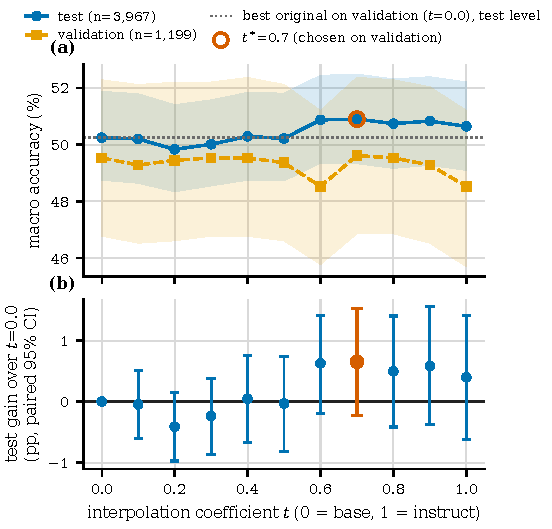
\includegraphics[width=\columnwidth]{figs/fig01_lerp_qwen.pdf}
\caption{(a) Macro accuracy along the base-to-instruct path: test (blue) and validation (orange, dashed) with 95\% CI bands; orange-red ring marks the validation-selected $t^\ast$, dotted line the test level of the better original. (b) Paired test gain over the better original, with 95\% CI. Every interval overlaps zero.}
\label{fig:lerp}
\end{figure}

\textbf{Primary result.} $\Delta=+0.65$ pp (95\% CI $[-0.23,+1.52]$, $p=0.149$). The interval contains zero, so the pre-registered criterion is not met and the outcome is a tie with the base model. Against the instruct model, $t^\ast$ gains $+0.25$ pp ($[-0.40,+0.92]$, $p=0.461$), also a tie. Since the nominal $p$ values are above 0.05, the Bonferroni threshold plays no role. The upper limit of the 95\% CI of the paired difference rules out a gain above $+1.52$ pp over the base model, by this selection procedure and this test set; a true gain of a few tenths of a point is compatible with the data.

\textbf{We cannot detect that the validation split ranks the coefficients.} Validation macro accuracy ranges from 48.53\% to 49.61\% over the grid, a spread of 1.1 pp, while each validation interval has a half-width of about 2.8 pp. Four coefficients ($t=0,0.3,0.4,0.8$) tie at 49.53\%, and $t=0.7$ wins at 49.61\%, a margin equal to one correctly classified item in one task. The same instruct-minus-base contrast has opposite sign on validation ($-1.00$ pp, $[-2.75,+0.92]$) and on test ($+0.40$ pp, $[-0.62,+1.41]$); both intervals contain zero. Across the eleven coefficients, the Spearman rank correlation between validation and test macro accuracy is $\rho=-0.03$ ($p=0.93$; \texttt{results/art01\_rank\_corr.txt}), so we detect no information in validation about the test ranking. With only eleven dependent points the interval on $\rho$ is wide, and $\rho\approx0$ is also what we would expect if all coefficients were equivalent on test. The selected coefficient is therefore essentially a draw among near-ties. It happens that $t=0.7$ is also the test maximum, which is a coincidence of this run and not evidence that selection worked.

\textbf{Shape of the test curve (descriptive).} Test macro accuracy is flat for $t\le0.5$ (49.83\% to 50.29\%) and roughly 0.5 pp higher for $t\ge0.6$ (50.64\% to 50.90\%). Every paired interval against the base model contains zero, including those of the five points with $t\ge0.6$ ($t=0.6,0.7,0.8,0.9,1.0$; differences $+0.40$ to $+0.65$ pp). At $t^\ast$ versus the base, per-task test accuracy moves by $+1.2$ pp on ARC-Easy, $+1.2$ pp on ARC-Challenge, $0.0$ pp on HellaSwag and $+0.2$ pp on WinoGrande; we computed no per-task intervals, and this decomposition is descriptive only.

\textbf{What cannot be concluded.} We cannot conclude that interpolation helps, or that it does not help by a fraction of a point. We cannot conclude that the instruct side of the path is better than the base side. We cannot extrapolate to other model pairs, sizes, benchmarks, or a chat-template evaluation.

\section{Discussion and Limitations}
\textbf{Interpretation.} The result is a null. One candidate reason is that the two endpoints are nearly interchangeable on these four benchmarks. The point estimates of instruct minus base are $-1.00$ pp on validation and $+0.40$ pp on test, and both intervals contain zero. Whether a path between such endpoints can exceed both is left open: \cite{wortsman2022wise} reports that it can in vision, and our interval for instruct minus base does not establish equivalence. We conjecture that this near-equivalence relates to the small size of the update: the norm of the instruct-minus-base difference is 4.18\% of the base-weight norm in this pair (exploratory, $\|\theta_i-\theta_b\|/\|\theta_b\|=0.0418$). We did not test this link. It also does not explain the vision results of \cite{wortsman2022wise}, which concern a different model class and objective.

\textbf{Precision.} All evaluations used bfloat16. Re-evaluating validation accuracy in fp32 at $t=0$, $0.7$ and $1$ lowered the macro accuracy by $0.67$, $0.41$ and $0.08$~pp (fp32: $0.4886$, $0.4920$, $0.4845$), a shift of the same size as the differences between coefficients, while the order of the three points did not change and WikiText-2 NLL moved by at most $0.0026$ nats at any $t$ (\texttt{results/fp32\_check\_qwen.txt}). Exact accuracy levels are therefore specific to bfloat16, and the test items were not re-evaluated in fp32.

\textbf{Threats to validity.} (i) Validation has only 300 items per task, and selection among eleven candidates on such a split is noisy; a larger validation set would sharpen the choice but not necessarily the gain. (ii) The test split is easier than validation (about 50.2\% vs.\ 49.5\% for the base model), so we compare gains between splits, not levels. (iii) The study covers a single model pair, a single scale ($\le0.5$B), four multiple-choice benchmarks scored by log-likelihood and one hardware platform. The instruct model is disadvantaged by the absence of a chat template. (iv) Possible benchmark contamination in either parent. (v) The grid step is 0.1, so a narrow optimum between grid points would be missed. (vi) One data split (seed 0). (vii) The paired bootstrap treats items as independent and ignores variability from the split itself.

\section{Conclusion}
For Qwen2.5-0.5B base and Instruct, validation-selected linear interpolation does not beat the better parent by more than noise: $+0.65$ pp, 95\% CI $[-0.23,+1.52]$ on 3{,}967 test items. The pre-registered hypothesis is not supported. For this pair, the 300-item validation split carried no detectable information about the test ranking of the eleven coefficients (Spearman $\rho=-0.03$, $p=0.93$; \texttt{results/art01\_rank\_corr.txt}). Calling a merged model better than its parents requires a paired interval, not a point estimate.

\section*{Data and Code Availability}
Code, per-item caches, tables and figures are in the project repository at git tag \texttt{preprints-v1} (the commit that contains this manuscript and all scripts and caches). The tables of this paper are regenerated by \texttt{experiments/art01\_06\_tables.py}; the rank correlation comes from \texttt{experiments/art01\_rank\_corr.py} (output \texttt{results/art01\_rank\_corr.txt}). Datasets: \texttt{allenai/ai2\_arc}, \texttt{Rowan/hellaswag}, \texttt{allenai/winogrande} (\texttt{winogrande\_xl}). Model revisions are listed above and in \texttt{MANIFEST.json}. Versions: Python 3.9.6, PyTorch 2.8.0, transformers 4.57.6, numpy 1.26.4, datasets 4.5.0. The single command \texttt{./run\_everything.sh} regenerates the curve and summaries (models and data are fetched by \texttt{common/baixar.py}). The pre-registration is \texttt{experiments/PREREG.md}, written before any merge was run.

\section*{Acknowledgments}
No external funding.

\begin{thebibliography}{99}
\bibitem{wortsman2022wise} M. Wortsman, G. Ilharco, J. W. Kim, et al., ``Robust fine-tuning of zero-shot models,'' in \emph{Proc.\ CVPR}, 2022, arXiv:2109.01903.
\bibitem{frankle2020lmc} J. Frankle, G. K. Dziugaite, D. M. Roy, et al., ``Linear mode connectivity and the lottery ticket hypothesis,'' in \emph{Proc.\ ICML}, 2020, arXiv:1912.05671.
\bibitem{izmailov2018swa} P. Izmailov, D. Podoprikhin, T. Garipov, et al., ``Averaging weights leads to wider optima and better generalization,'' in \emph{Proc.\ UAI}, 2018, arXiv:1803.05407.
\bibitem{wortsman2022soups} M. Wortsman, G. Ilharco, S. Y. Gadre, et al., ``Model soups: averaging weights of multiple fine-tuned models improves accuracy without increasing inference time,'' in \emph{Proc.\ ICML}, 2022, arXiv:2203.05482.
\bibitem{rame2023rewarded} A. Ram\'e, G. Couairon, M. Shukor, et al., ``Rewarded soups: towards Pareto-optimal alignment by interpolating weights fine-tuned on diverse rewards,'' in \emph{NeurIPS}, 2023, arXiv:2306.04488.
\bibitem{shoemake1985slerp} K. Shoemake, ``Animating rotation with quaternion curves,'' in \emph{SIGGRAPH}, 1985, doi:10.1145/325165.325242.
\bibitem{ainsworth2023rebasin} S. K. Ainsworth, J. Hayase, and S. Srinivasa, ``Git Re-Basin: merging models modulo permutation symmetries,'' in \emph{ICLR}, 2023, arXiv:2209.04836.
\bibitem{matena2022fisher} M. Matena and C. Raffel, ``Merging models with Fisher-weighted averaging,'' in \emph{NeurIPS}, 2022, arXiv:2111.09832.
\bibitem{jin2023dataless} X. Jin, X. Ren, D. Preotiuc-Pietro, et al., ``Dataless knowledge fusion by merging weights of language models,'' in \emph{Proc.\ ICLR}, 2023, arXiv:2212.09849.
\bibitem{ilharco2023taskarith} G. Ilharco, M. T. Ribeiro, M. Wortsman, et al., ``Editing models with task arithmetic,'' in \emph{Proc.\ ICLR}, 2023, arXiv:2212.04089.
\bibitem{yadav2023ties} P. Yadav, D. Tam, L. Choshen, et al., ``TIES-Merging: resolving interference when merging models,'' in \emph{NeurIPS}, 2023, arXiv:2306.01708.
\bibitem{yu2024dare} L. Yu, B. Yu, H. Yu, et al., ``Language models are Super Mario: absorbing abilities from homologous models as a free lunch,'' in \emph{Proc.\ ICML}, 2024, arXiv:2311.03099.
\bibitem{yang2024survey} E. Yang, L. Shen, G. Guo, et al., ``Model merging in LLMs, MLLMs, and beyond: methods, theories, applications and opportunities,'' arXiv:2408.07666, 2024.
\bibitem{li2023fusion} W. Li, Y. Peng, M. Zhang, et al., ``Deep model fusion: a survey,'' arXiv:2309.15698, 2023.
\bibitem{yadav2024scale} P. Yadav, T. Vu, J. Lai, et al., ``What matters for model merging at scale?'' arXiv:2410.03617, 2024.
\bibitem{huang2023chatvector} S.-C. Huang, P.-Z. Li, Y.-C. Hsu, et al., ``Chat Vector: a simple approach to equip LLMs with instruction following and model alignment in new languages,'' in \emph{Proc.\ ACL}, 2024, arXiv:2310.04799.
\bibitem{goddard2024mergekit} C. Goddard, S. Siriwardhana, M. Ehghaghi, et al., ``Arcee's MergeKit: a toolkit for merging large language models,'' arXiv:2403.13257, 2024.
\bibitem{dwork2015adaptive} C. Dwork, V. Feldman, M. Hardt, et al., ``Preserving statistical validity in adaptive data analysis,'' arXiv:1411.2664, 2014.
\bibitem{miller2024errorbars} E. Miller, ``Adding error bars to evals: a statistical approach to language model evaluations,'' arXiv:2411.00640, 2024.
\bibitem{qwen2024qwen25} Qwen, A. Yang, et al., ``Qwen2.5 technical report,'' arXiv:2412.15115, 2024.
\bibitem{clark2018arc} P. Clark, I. Cowhey, O. Etzioni, et al., ``Think you have solved question answering? Try ARC, the AI2 Reasoning Challenge,'' arXiv:1803.05457, 2018.
\bibitem{zellers2019hellaswag} R. Zellers, A. Holtzman, Y. Bisk, et al., ``HellaSwag: can a machine really finish your sentence?'' in \emph{Proc.\ ACL}, 2019, arXiv:1905.07830.
\bibitem{sakaguchi2020winogrande} K. Sakaguchi, R. Le Bras, C. Bhagavatula, et al., ``WinoGrande: an adversarial Winograd schema challenge at scale,'' in \emph{AAAI}, 2020, arXiv:1907.10641.
\bibitem{efron1979bootstrap} B. Efron, ``Bootstrap methods: another look at the jackknife,'' \emph{Ann. Statist.}, vol.~7, no.~1, 1979, doi:10.1214/aos/1176344552.
\bibitem{gao2023harness} L. Gao et al., ``EleutherAI/lm-evaluation-harness,'' Zenodo, doi:10.5281/zenodo.10256836.
\bibitem{santos2026modelmergingfo} D. F. Santos, ``Model Merging for Capability Composition: A Technical Note,'' Zenodo, 2026, doi:10.5281/zenodo.21610555.
\bibitem{santos2026collapseresist} D. F. Santos, ``Collapse-Resistant Joint-Embedding Predictive Architectures: A Controlled Comparison of SIGReg, VICReg, and EMA,'' Zenodo, v2, 2026, doi:10.5281/zenodo.24223364.
\bibitem{santos2026knowledgedisti} D. F. Santos, ``Knowledge Distillation and Self-Distillation for Language Models,'' Zenodo, 2026, doi:10.5281/zenodo.21610100.
\bibitem{santos2026parametereffic} D. F. Santos, ``Parameter-Efficient Fine-Tuning: LoRA, QLoRA, and DoRA,'' Zenodo, 2026, doi:10.5281/zenodo.21610033.
\bibitem{santos2026mixtureofexper} D. F. Santos, ``Mixture-of-Experts Training and Sparse Upcycling,'' Zenodo, 2026, doi:10.5281/zenodo.21610062.
\bibitem{santos2026curriculumlear} D. F. Santos, ``Curriculum Learning and Data-Efficient Pretraining: A Technical Note,'' Zenodo, 2026, doi:10.5281/zenodo.21610595.
\bibitem{santos2026syntheticdatag} D. F. Santos, ``Synthetic Data Generation and Self-Improvement: A Technical Note,'' Zenodo, 2026, doi:10.5281/zenodo.21610525.
\bibitem{santos2026directpreferen} D. F. Santos, ``Direct Preference Optimization (DPO): A Technical Note,'' Zenodo, 2026, doi:10.5281/zenodo.21609911.
\bibitem{santos2026rlaifandconsti} D. F. Santos, ``RLAIF and Constitutional AI: A Technical Note,'' Zenodo, 2026, doi:10.5281/zenodo.21610280.
\bibitem{santos2026reinforcementl} D. F. Santos, ``Reinforcement Learning with Verifiable Rewards (RLVR) and GRPO for Reasoning,'' Zenodo, 2026, doi:10.5281/zenodo.21609980.
\end{thebibliography}

\end{document}
